\documentclass[aspectratio=169]{beamer}

\usetheme{Boadilla}
\usefonttheme{professionalfonts}
\setbeamertemplate{navigation symbols}{}
\setbeamertemplate{itemize items}[circle]
\setbeamertemplate{enumerate items}[default]
\setbeamertemplate{headline}{}

\usepackage[utf8]{inputenc}
\usepackage[T1]{fontenc}
\usepackage{lmodern}
\usepackage{amsmath}
\usepackage{booktabs}
\usepackage{tabularx}
\usepackage{array}
\usepackage{hyperref}
\usepackage[strings]{underscore}
\usepackage{listings}
\usepackage{tikz}
\usetikzlibrary{arrows.meta,positioning,fit,calc,shapes.geometric}
\usepackage{xcolor}

\definecolor{courseblue}{HTML}{12355B}
\definecolor{coursegold}{HTML}{C98A2E}
\definecolor{courseice}{HTML}{EEF3F8}
\definecolor{coursegreen}{HTML}{2F6B4F}
\definecolor{coursegray}{HTML}{4B5563}
\definecolor{codebg}{HTML}{F7F9FC}
\definecolor{codecomment}{HTML}{5E6C84}
\definecolor{codestring}{HTML}{0B6E4F}

\setbeamercolor{palette primary}{bg=courseblue,fg=white}
\setbeamercolor{palette secondary}{bg=coursegold,fg=white}
\setbeamercolor{palette tertiary}{bg=courseblue,fg=white}
\setbeamercolor{palette quaternary}{bg=coursegold,fg=white}
\setbeamercolor{structure}{fg=courseblue}
\setbeamercolor{frametitle}{bg=courseice,fg=courseblue}
\setbeamercolor{title}{fg=courseblue}
\setbeamercolor{block title}{bg=courseblue,fg=white}
\setbeamercolor{block body}{bg=courseice,fg=black}
\setbeamercolor{normal text}{fg=black,bg=white}
\setbeamercolor{alerted text}{fg=coursegold}

\setbeamerfont{footline}{size=\scriptsize}

\setbeamertemplate{footline}{
  \leavevmode
  \hbox{
    \begin{beamercolorbox}[wd=.33\paperwidth,ht=2.8ex,dp=1.2ex,leftskip=0.8em]{palette primary}%
      University of Trieste
    \end{beamercolorbox}%
    \begin{beamercolorbox}[wd=.49\paperwidth,ht=2.8ex,dp=1.2ex,center]{palette tertiary}%
      \coursename{} \textbar{} \coursecode
    \end{beamercolorbox}%
    \begin{beamercolorbox}[wd=.18\paperwidth,ht=2.8ex,dp=1.2ex,right,rightskip=0.8em]{palette secondary}%
      \insertframenumber{} / \inserttotalframenumber
    \end{beamercolorbox}%
  }
}

\hypersetup{
  colorlinks=true,
  linkcolor=courseblue,
  urlcolor=coursegreen
}

\lstdefinestyle{coursepython}{
  language=Python,
  basicstyle=\ttfamily\footnotesize,
  keywordstyle=\color{courseblue}\bfseries,
  commentstyle=\color{codecomment}\itshape,
  stringstyle=\color{codestring},
  showstringspaces=false,
  columns=fullflexible,
  keepspaces=true,
  frame=single,
  framerule=0.6pt,
  rulecolor=\color{courseblue},
  backgroundcolor=\color{codebg},
  xleftmargin=0.4em,
  xrightmargin=0.4em,
  aboveskip=0.4em,
  belowskip=0.2em
}

\newcommand{\coursename}{Data-driven Systems Engineering}
\newcommand{\coursecode}{440MI / 305SM}
\newcommand{\coursefooter}{}

\newcommand{\learninggoals}[1]{
  \begin{block}{Learning goals}
  #1
  \end{block}
}

\newcommand{\repoactivity}[1]{
  \begin{block}{Repo activity}
  #1
  \end{block}
}

\newcommand{\readinglist}[1]{
  \begin{block}{Papers and materials}
  {\footnotesize #1}
  \end{block}
}

\newcommand{\coursecontextframe}[5]{
  \begin{frame}{Course Map and Running Cases}
  \centering
  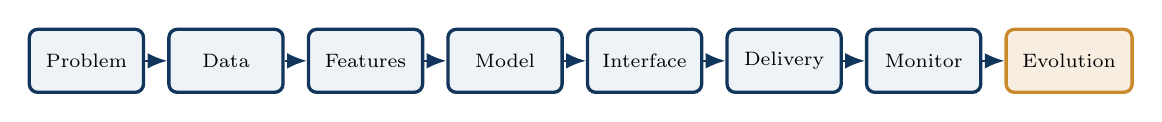
\begin{tikzpicture}[node distance=0.28cm]
  \node[flowbox, minimum width=1.45cm, minimum height=0.8cm] (problem) {\scriptsize Problem};
  \node[flowbox, minimum width=1.45cm, minimum height=0.8cm, right=of problem] (data) {\scriptsize Data};
  \node[flowbox, minimum width=1.45cm, minimum height=0.8cm, right=of data] (features) {\scriptsize Features};
  \node[flowbox, minimum width=1.45cm, minimum height=0.8cm, right=of features] (model) {\scriptsize Model};
  \node[flowbox, minimum width=1.45cm, minimum height=0.8cm, right=of model] (interface) {\scriptsize Interface};
  \node[flowbox, minimum width=1.45cm, minimum height=0.8cm, right=of interface] (delivery) {\scriptsize Delivery};
  \node[flowbox, minimum width=1.45cm, minimum height=0.8cm, right=of delivery] (monitor) {\scriptsize Monitor};
  \node[accentbox, minimum width=1.6cm, minimum height=0.8cm, right=of monitor] (evolution) {\scriptsize Evolution};
  \foreach \a/\b in {problem/data,data/features,features/model,model/interface,interface/delivery,delivery/monitor,monitor/evolution} {
    \draw[arrow] (\a) -- (\b);
  }
  \end{tikzpicture}

  \vspace{0.5em}
  \begin{block}{Today in the course}
  \textbf{Focus:} #1

  \textbf{Bridge:} #2
  \end{block}

  \begin{columns}[T]
  \column{0.48\textwidth}
  \begin{block}{Fraud case}
  {\footnotesize #3}
  \end{block}
  \column{0.48\textwidth}
  \begin{block}{Pasteurization case}
  {\footnotesize #4}
  \end{block}
  \end{columns}

  \vspace{0.3em}
  {\footnotesize \textbf{Course thread:} #5}
  \coursefooter
  \end{frame}
}

\newcommand{\classclosingframe}[4]{
  \begin{frame}{From This Class to the Next}
  \begin{block}{What stays with us}
  #1
  \end{block}

  \begin{columns}[T]
  \column{0.48\textwidth}
  \begin{block}{Project use}
  {\footnotesize #2}
  \end{block}
  \column{0.48\textwidth}
  \begin{block}{Next connection}
  {\footnotesize #3}
  \end{block}
  \end{columns}

  \vspace{0.3em}
  {\footnotesize \textbf{Course thread:} #4}
  \coursefooter
  \end{frame}
}

\tikzset{
  flowbox/.style={
    rounded corners=3pt,
    draw=courseblue,
    fill=courseice,
    very thick,
    minimum width=2.2cm,
    minimum height=0.9cm,
    align=center,
    font=\small
  },
  accentbox/.style={
    rounded corners=3pt,
    draw=coursegold,
    fill=coursegold!15,
    very thick,
    minimum width=2.2cm,
    minimum height=0.9cm,
    align=center,
    font=\small
  },
  arrow/.style={
    -{Latex[length=2.5mm,width=2mm]},
    thick,
    draw=courseblue
  }
}

\usepackage{amssymb}

\title{Class 18: Online Learning and Concept Drift}
\author{\coursename}
\date{}

\begin{document}

\frame{\titlepage \coursefooter}

\begin{frame}{Agenda}
\begin{itemize}
\item Why a validated model can become obsolete.
\item Offline (batch) versus online (incremental) learning.
\item River: learning one observation at a time, with prequential evaluation.
\item Concept drift: definition, types, and detection with ADWIN.
\item Monitoring a streaming model with River and Evidently.
\end{itemize}
\coursefooter
\end{frame}

\begin{frame}{Offline versus online learning}
\begin{columns}[T]
\column{0.48\textwidth}
\textbf{Offline (batch)}
\begin{itemize}
\item Trained once on a fixed dataset $\mathcal{D} = \{(\mathbf{x}_i, y_i)\}_{i=1}^{n}$.
\item Straightforward benchmarking on a held-out test set.
\item Adapts only through periodic retraining.
\end{itemize}
\column{0.48\textwidth}
\textbf{Online (incremental)}
\begin{itemize}
\item Updated after each observation $(\mathbf{x}_t, y_t)$ of a stream, with constant memory.
\item Operates directly on unbounded data streams.
\item Adapts continuously to change.
\end{itemize}
\end{columns}
\vspace{0.6em}
\begin{itemize}
\item \textbf{Prequential evaluation} (test-then-train): each observation is first used to test the model, $\hat{y}_t = f_{t-1}(\mathbf{x}_t)$, and only then to update it, so every prediction is made on unseen data.
\end{itemize}
\coursefooter
\end{frame}

\begin{frame}{Why adaptation becomes necessary}
\begin{itemize}
\item User behaviour changes.
\item Sensors degrade or are recalibrated.
\item Business policies or regulations change.
\item New error types appear only after deployment.
\end{itemize}
\begin{block}{Key point}
Adaptation does not indicate that the initial model was wrong; it acknowledges that the data-generating process evolves over time.
\end{block}
\coursefooter
\end{frame}

\begin{frame}[fragile]{River example: incremental regression}
\begin{lstlisting}[style=coursepython]
model = preprocessing.StandardScaler() | linear_model.LinearRegression(
    optimizer=optim.SGD(0.01)
)
mae = metrics.MAE()

y_pred = model.predict_one(x)
model.learn_one(x, y)
mae.update(y, y_pred)
\end{lstlisting}
\begin{itemize}
\item From \texttt{notebooks/Class8\_Model\_Incremental\_learning.ipynb}: the model predicts the current temperature in Paris from the wind speed (\texttt{x = \{"wind": wind\}}), obtained from the Open-Meteo API, which refreshes these values every 15 minutes; polling faster only repeats the same observation.
\item \texttt{predict\_one} precedes \texttt{learn\_one} (prequential evaluation); the mean absolute error (MAE) and the parameters, by stochastic gradient descent (SGD), are updated at every observation.
\end{itemize}
\coursefooter
\end{frame}

\begin{frame}{What is concept drift?}
\begin{itemize}
\item Concept drift is a change over time of the joint distribution, $P_t(\mathbf{x}, y) \neq P_{t+\Delta}(\mathbf{x}, y)$; it is a change of the data-generating process, not noise in individual readings.
\item Since $P(\mathbf{x}, y) = P(\mathbf{x})\,P(y \mid \mathbf{x})$, two cases are distinguished:
\begin{itemize}
\item \textbf{virtual drift} (covariate shift): $P(\mathbf{x})$ changes, $P(y \mid \mathbf{x})$ does not;
\item \textbf{real drift}: $P(y \mid \mathbf{x})$ changes, so the learned decision function becomes incorrect.
\end{itemize}
\item A model trained before a real drift may still produce confident predictions that are systematically wrong.
\end{itemize}
\coursefooter
\end{frame}

\begin{frame}{Virtual versus real drift}
\centering
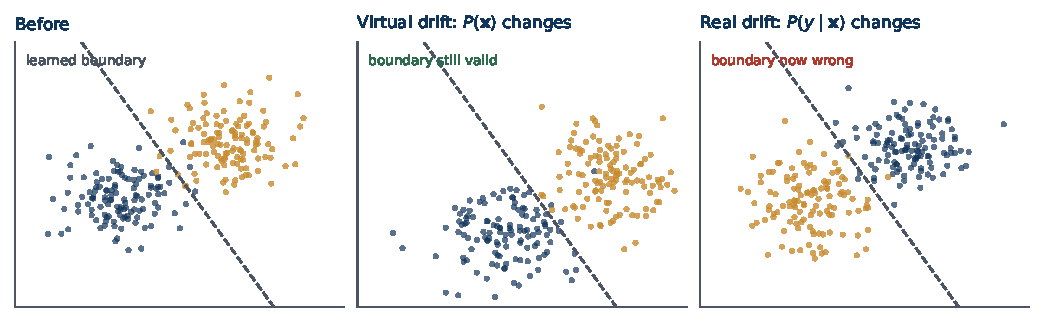
\includegraphics[width=\textwidth,height=0.48\textheight,keepaspectratio]{images/class18_virtual_real_drift.pdf}

\vspace{0.3em}
\begin{itemize}\footnotesize
\item \textbf{Virtual drift:} the inputs move to a different region of $\mathcal{X}$, but the class of each point is unchanged; the learned boundary remains correct, although the model may now operate where it saw little training data.
\item \textbf{Real drift:} the same inputs now belong to the other class; the boundary itself is wrong and the model must be updated.
\item Monitoring the inputs alone (e.g.\ a data drift report) detects virtual drift; detecting real drift requires the labels, i.e.\ the error stream.
\end{itemize}
{\tiny Illustrative synthetic data.\par}
\coursefooter
\end{frame}

\begin{frame}{Temporal patterns of drift}
\centering
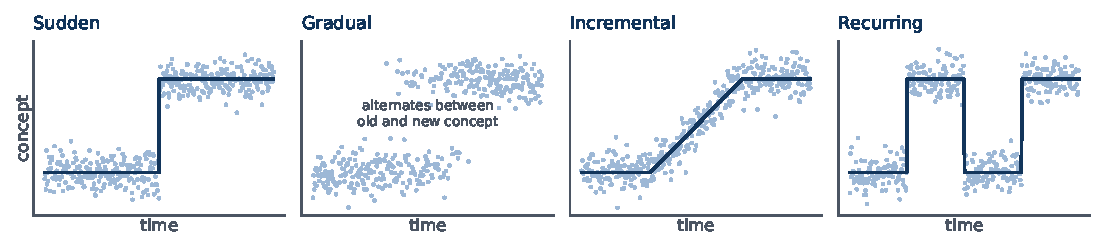
\includegraphics[width=\textwidth]{images/class18_drift_types.pdf}

\vspace{0.4em}
\begin{itemize}\footnotesize
\item \textbf{Sudden:} the concept is replaced at once, e.g.\ a sensor recalibration or a change of product.
\item \textbf{Gradual:} samples from the old and the new concept alternate, with the new one becoming more frequent.
\item \textbf{Incremental:} the concept moves continuously through intermediate states, e.g.\ wear of heating equipment.
\item \textbf{Recurring:} previous concepts return, e.g.\ seasonal patterns; a model can reuse what it learned before.
\end{itemize}
{\tiny Illustrative synthetic data; dots are observations, lines the underlying concept.\par}
\coursefooter
\end{frame}

\begin{frame}{The streaming learning loop}
\centering
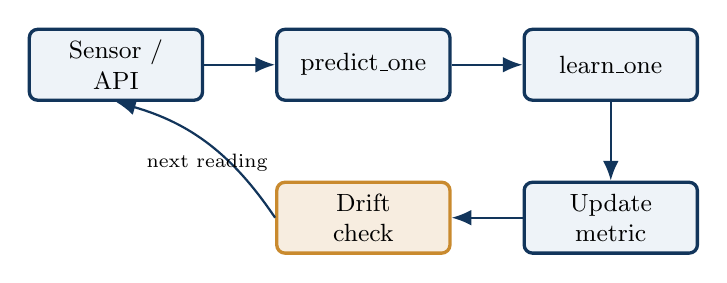
\begin{tikzpicture}[node distance=1cm and 0.9cm]
\node[flowbox] (source) {Sensor /\\API};
\node[flowbox, right=of source] (predict) {predict\_one};
\node[flowbox, right=of predict] (learn) {learn\_one};
\node[flowbox, below=of learn] (metric) {Update\\metric};
\node[accentbox, left=of metric] (drift) {Drift\\check};
\draw[arrow] (source) -- (predict);
\draw[arrow] (predict) -- (learn);
\draw[arrow] (learn) -- (metric);
\draw[arrow] (metric) -- (drift);
\draw[arrow, bend right=20] (drift.west) to node[below, font=\scriptsize] {next reading} (source.south);
\end{tikzpicture}
\coursefooter
\end{frame}

\begin{frame}[fragile]{River example: ADWIN drift detection}
\begin{lstlisting}[style=coursepython]
adwin = drift.ADWIN(delta=0.002)
...
error = abs(y - (y_pred or 0))
adwin.update(error)

if adwin.drift_detected:
    print("Resetting model due to detected drift...")
    model = preprocessing.StandardScaler() | linear_model.LinearRegression(
        optimizer=optim.SGD(0.01)
    )
    adwin = drift.ADWIN(delta=0.002)
\end{lstlisting}
\begin{itemize}
\item From \texttt{notebooks/Class8\_Model\_Incremental\_learning.ipynb}: the adaptive windowing detector (ADWIN) monitors the absolute errors and signals a significant change; the notebook then resets both the model and the detector, a strategy examined experimentally below.
\end{itemize}
\coursefooter
\end{frame}

\begin{frame}{How ADWIN works}
\begin{itemize}
\item ADWIN (Bifet and Gavald\`a, 2007) maintains a window $W$ of the most recent values (here, absolute errors) and examines every split of $W$ into an older part $W_0$ and a recent part $W_1$, of sizes $n_0$ and $n_1$.
\item A change is detected, and $W_0$ is dropped, when the two means differ by more than a threshold derived from the Hoeffding bound:
\[
|\hat{\mu}_{W_0} - \hat{\mu}_{W_1}| \ge \varepsilon_{\mathrm{cut}}, \qquad
\varepsilon_{\mathrm{cut}} = \sqrt{\frac{1}{2m}\ln\frac{4}{\delta'}}, \quad
m = \frac{1}{1/n_0 + 1/n_1}, \quad \delta' = \frac{\delta}{n}.
\]
\item The confidence parameter $\delta$ (here $0.002$) controls the false-alarm rate: the window grows while the stream is stable and shrinks as soon as its mean changes.
\item This provides a statistically grounded trigger for retraining or resetting, instead of a fixed retraining schedule.
\end{itemize}
\coursefooter
\end{frame}

\begin{frame}{ADWIN on the pasteurization stream}
\begingroup\small
\textbf{Experiment:} an online soft sensor estimates the viscosity $\eta$ from the temperature $T$ (60 batches, 19{,}530 samples at 1\,Hz). After batch 30, a product change raises $\eta$ by 0.4\,cP at every temperature: a sudden real drift.
\par\endgroup
\vspace{0.3em}
\centering
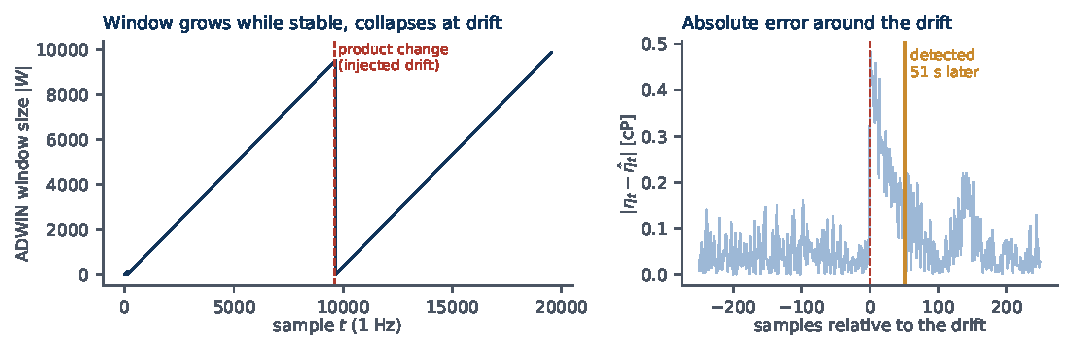
\includegraphics[width=\textwidth,height=0.45\textheight,keepaspectratio]{images/class18_adwin_detection.pdf}

\vspace{0.2em}
\begin{itemize}\footnotesize
\item The ADWIN window grows linearly while the error stream is stationary and collapses when the drift is detected, 51 samples (51\,s) after it occurred.
\item Apart from one alarm during the initial learning phase, no false alarm is raised in 19{,}530 samples ($\delta = 0.002$).
\end{itemize}
{\tiny Data from \texttt{pasteurization/synth\_sensors.py} with an injected drift; River 0.22, \texttt{LinearRegression} with SGD, \texttt{ADWIN(delta=0.002)}.\par}
\coursefooter
\end{frame}

\begin{frame}{Adaptation strategies compared}
\centering
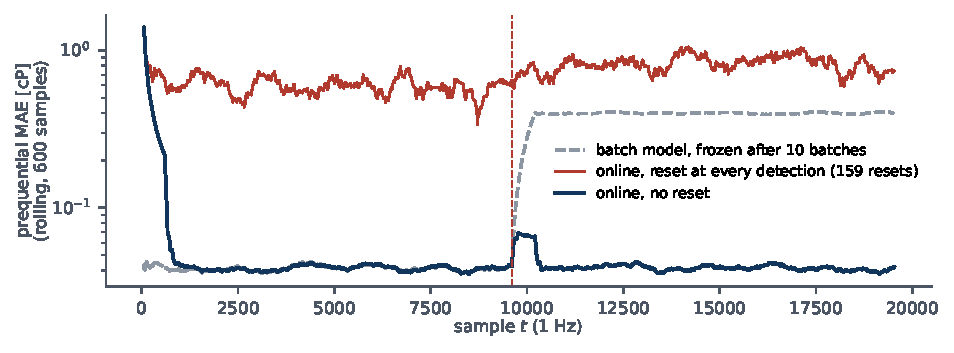
\includegraphics[width=\textwidth,height=0.45\textheight,keepaspectratio]{images/class18_adaptation_strategies.pdf}

\vspace{0.2em}
\begingroup\footnotesize
\begin{tabular}{l c c l}
Strategy & MAE before & MAE after & \\
\toprule
Batch model, frozen after 10 batches & 0.041 & 0.398 & does not adapt \\
Online, no reset & 0.052 & 0.043 & recovers in about 200 samples (3.5 min) \\
Online, reset at every detection & 0.599 & 0.820 & 159 resets: reset loop \\
\bottomrule
\end{tabular}
\par\endgroup
\vspace{0.3em}
\begin{itemize}\footnotesize
\item A reset replaces the model by an untrained one, whose large and decreasing error is itself a change that ADWIN detects: the model never stabilizes. Safer responses are to warm-start from the current model, retrain on the recent window $W_1$, or only raise an alert.
\end{itemize}
\coursefooter
\end{frame}

\begin{frame}{Monitoring beyond a single detector}
\begin{itemize}
\item \texttt{notebooks/Class8\_Model\_Incremental\_learning.ipynb} also produces Evidently reports (\texttt{DataDriftPreset}, \texttt{DataQualityPreset}) alongside River.
\item ADWIN on the error stream is a fast, targeted signal that detects degradation of performance; a drift report tests the distribution of every input column and can reveal virtual drift before performance degrades.
\item Combining a lightweight online detector with periodic, more comprehensive reports is a common production pattern.
\end{itemize}
\coursefooter
\end{frame}

\begin{frame}{Batch retraining versus online learning}
\begin{tabularx}{\textwidth}{>{\bfseries}l X}
Latency of adaptation & Online learning adapts immediately; batch retraining waits for the next cycle. \\
\addlinespace[0.3em]
Auditability & Batch models are fixed snapshots that can be reviewed and versioned; the state of an online model changes continuously. \\
\addlinespace[0.3em]
Stability & Online models may overreact to noise if the detector or the learning rate is too sensitive. \\
\addlinespace[0.3em]
Infrastructure & Online learning avoids large periodic training jobs but requires an always-on service. \\
\bottomrule
\end{tabularx}
\coursefooter
\end{frame}

\begin{frame}{Drift in the two running cases}
\begin{itemize}
\item \textbf{Fraud:} seasonal spending patterns and new merchant categories (virtual drift); fraudsters adopting new tactics (real drift).
\item \textbf{Pasteurization:} sensor recalibration (sudden), raw-material variability, or wear of heating and cooling equipment (gradual).
\item In both cases, drift detection turns ``the model has become worse'' from an unexplained observation into a specific, timestamped event.
\end{itemize}
\coursefooter
\end{frame}

\begin{frame}{Repository connections}
\repoactivity{
\begin{itemize}
\item \texttt{notebooks/Class8\_Model\_Incremental\_learning.ipynb}: River regression, ADWIN, and Evidently reports.
\item \texttt{streamlit/pages/App\_Stream.py}: the same River and ADWIN pattern as a live dashboard, plotting detected change points on the MAE curve.
\end{itemize}
}
\coursefooter
\end{frame}

\begin{frame}{Papers and materials}
\readinglist{
\fontsize{6.8}{8.2}\selectfont
\begin{columns}[T]
\column{0.5\textwidth}
\begin{itemize}\setlength{\itemsep}{1pt}
\item Gama, J., \v{Z}liobait\.{e}, I., Bifet, A., Pechenizkiy, M., Bouchachia, A. (2014). A survey on concept drift adaptation. \emph{ACM Computing Surveys}, 46(4), 44:1--44:37.
\item Bifet, A., Gavald\`a, R. (2007). Learning from time-changing data with adaptive windowing. \emph{Proceedings of the SIAM International Conference on Data Mining}, 443--448.
\item Lu, J., Liu, A., Dong, F., Gu, F., Gama, J., Zhang, G. (2019). Learning under concept drift: A review. \emph{IEEE Transactions on Knowledge and Data Engineering}, 31(12), 2346--2363.
\end{itemize}
\column{0.5\textwidth}
\begin{itemize}\setlength{\itemsep}{1pt}
\item Montiel, J., et al.\ (2021). River: machine learning for streaming data in Python. \emph{Journal of Machine Learning Research}, 22(110), 1--8.
\item Gama, J., Sebasti\~ao, R., Rodrigues, P.\,P. (2013). On evaluating stream learning algorithms. \emph{Machine Learning}, 90(3), 317--346.
\item Documentation: \href{https://riverml.xyz/latest/}{River}; \href{https://docs.evidentlyai.com/}{Evidently}.
\end{itemize}
\end{columns}
}
\coursefooter
\end{frame}

\begin{frame}{Take-away message}
\vfill
\centering
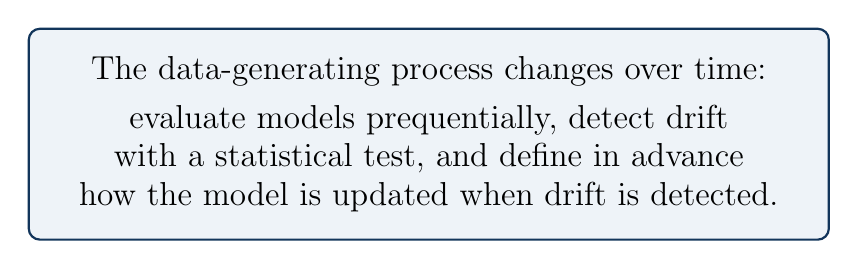
\begin{tikzpicture}
\node[fill=courseice, draw=courseblue, thick, rounded corners=4pt, inner sep=10pt, text width=0.78\textwidth, align=center, font=\large] {The data-generating process changes over time:\\[0.3em] evaluate models prequentially, detect drift\\ with a statistical test, and define in advance\\ how the model is updated when drift is detected.};
\end{tikzpicture}

\vfill
{\Large\bfseries\color{courseblue} Thank you for your attention.}

\vspace{0.4em}
{\small\color{coursegray} Next: Class 19 --- hands-on lab: streaming the pasteurization sensors.}
\vfill
\coursefooter
\end{frame}

\end{document}
